\documentclass[12pt]{article}

% for footnotes
\makeatletter
\newcommand\footnoteref[1]{\protected@xdef\@thefnmark{\ref{#1}}\@footnotemark}
\makeatother

\usepackage{common}
\usepackage{macros}
\usepackage{nameref}
\usepackage{pdflscape}
\newcommand{\sts}{Seq2Seq}
\newcommand{\embed}{\mathsf{embed}}
\title{HW3: Neural Machine Translation}
\author{Jiafeng Chen \and Yufeng Ling \and
Francisco Rivera}

\begin{document}

\maketitle

\section{Introduction}
In this writeup we consider neural machine translation---given a source sentence in one language, can we generate a target sentence in another? We work with the prevailing encoder-decoder architecture, where one neural network, the \emph{encoder}, maps the source sentence into a numerical tensor---which is supposed to be a latent representation of the source sentence. Another network, the \emph{decoder}, is a language model that takes the encoded sentence as an input, and generates a sentence in the target language. 

\section{Problem Description}
In this writeup, we consider the problem of machine translation. Let 
\begin{equation}
	\bm x_i = [x_{i1},\ldots,x_{iS}]
\end{equation}
be a source sentence, where each word belongs to some source vocabulary, $x_{it} \in \mathcal V_s$. Let 
\begin{equation}
	\bm y_i = [y_{i1},\ldots,y_{iT}]
\end{equation}
be a target sentence, with each target word belonging to some target vocabulary, $y_{it} \in \mathcal V_t$. Our goal is to learn $p(\bm y_i \mid \bm x_i)$. We often treat the prediction like a language model---i.e. we consider the sequential conditional distributions $p(y_{it} \mid y_{i1},\ldots,y_{i,t-1}, \bm x_i)$.


\section{Model and Algorithms}

\subsection{Sequence-to-Sequence (\sts)}
\label{sub:seq2seq}
In \sts{} (\cite{sutskever2014sequence}), we have a encoder-decoder network architecture. The \emph{encoder}, in the vanilla \sts{} implementation, is an LSTM network that takes an embedding of the source sentence $\embed(\bm x_{i1}),\ldots,\embed(\bm x_{iS})$ and outputs a list of hidden states $\bm h_{i1},\ldots, \bm h_{iS}$ and cell state $\bm c_{iS}$.

In \sts{}, the decoder is another LSTM which is initialized with $\bm h_{iS}$ and $\bm c_{iS}$. At training time, the decoder LSTM takes embeddings of the ground truth target $\embed(y_{it})$ and output probability predictions for $y_{i,t+1}$. These predictions are penalized with the usual cross entropy loss at training time. At prediction time, the decoder LSTM gets passed the start-of-sentence token \texttt{<s>} and outputs predictions for the first word. We then iteratively pass in its top predictions to obtain predictions for future words. For instance, a greedy algorithm to generate a sentence would be taking the top prediction every time and pass the predicted sentence so far into the decoder to obtain the next word---stopping when the end-of-sentence token \texttt{</s>} is the top prediction.\footnote{This corresponds to beam search with beam size 1.}  

\subsection{Attention}
\label{sub:attn}
The attention model (\cite{vaswani2017attention}) builds upon the Sequence-to-Sequence model described in section (\ref{sub:seq2seq}). Instead of only using the end state of the encoded input as input, we take advantage of a bi-directional RNN and generate target sentence by taking in a weighted input of all the states of the encoder. The intuition is that when we are translating a sentence, the adjacent words of the current word also help inform how we should translate the current word. Such weighted average is aptly named ``context''. To formalize this, we let the sequential conditional distribution be given by
\begin{equation}
	p(y_{it} \mid y_{i1}, \dots, y_{i,t-1}, \bm x_i) = g(y_{i,t-1}, s_t, c_t)
\end{equation}
where $s_t$ is the hidden state from BiRNN at time $t$ defined by
\begin{equation}
	s_t = f(s_{t-1}, y_{i,t-1}, c_t).
\end{equation}
As mentioned above, the context vector $c_t$ is a weighted average given by
\begin{equation}
	c_t = \sum_{j=1}^{T_x} \alpha_{tj} h_j
\end{equation}
where the annotations $\{h_j\}$ are the concatenated hidden states of the BiRNN and $\{\alpha_{tj}\}$ are the weights, which usually center around the current state $t$. The weights 
\begin{equation}
	\alpha_{tj} = \frac{\exp(e_{tj})}{\sum_{k=1}^{T_x} \exp(e_tk)}
\end{equation}
are generated by softmaxing over
\begin{equation}
	e_{tk} = a(s_{t-1}, h_k)
\end{equation}
for some function $a$. In our model, we take $a$ to be the dot product between the two arguments.

\begin{figure}
	\centering
	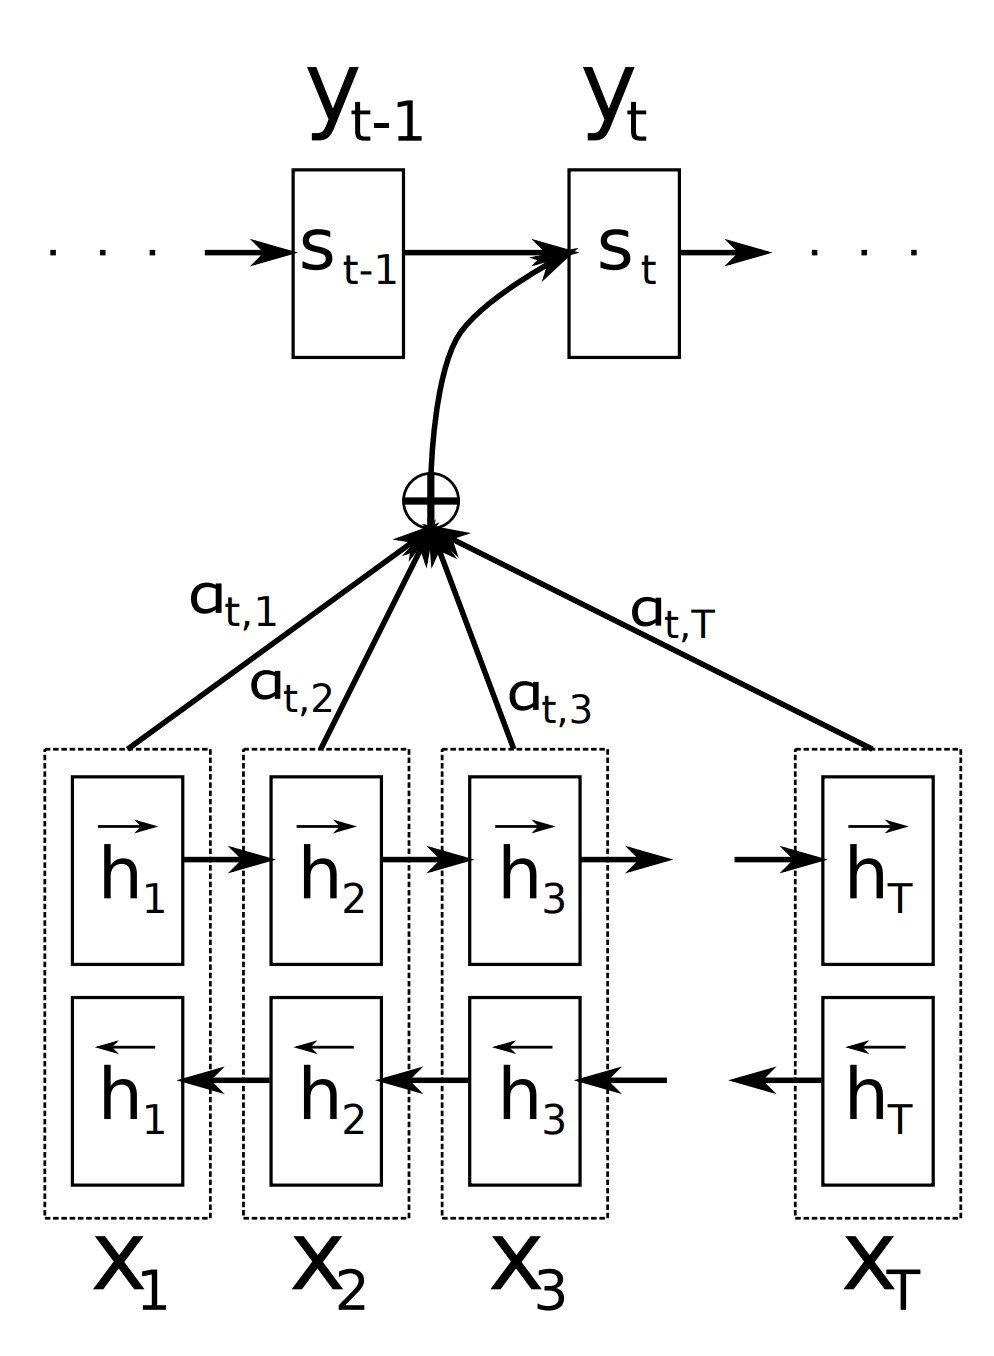
\includegraphics[width=0.3\linewidth]{figs/attn_diagram}
	\caption{Attention Diagram}
	\label{attn_diagram}
\end{figure}


\subsection{Beam Search}
\label{sub:beam}
After we have trained a model, since the outputs are conditional probabilities over the entire vocabulary, we need to have an algorithm that generates the top $k$ most likely sentences. One can use the greedy algorithm by selecting the local MLE conditional on the previously selected words. However, this can easily run into problems like stucking at a local optimum.

Beam search is proposed based on this idea. Instead of selecting the MLE, we select the top $B$ words with the largest conditional probabilities. The parameter $B$ is known as the ``beam width''. At every step, we choose the top $B$ words with the highest joint probability conditional on the $B$ previously generated sentenses $\{\bm y_{i, 1:t-1}^{(b)}\}_{b=1}^B$. That is
\begin{align}
	&\arg \max_{y_{it}, b} p(y_{it}, y_{i,t-1}^{(b)}, \dots, y_{i1}^{(b)}, \bm x_i)\nonumber = \arg \max_{y_{it}, b} p(y_{it} \mid y_{i,t-1}^{(b)}, \dots, y_{i1}^{(b)}, \bm x_i) p(y_{i,t-1}^{(b)}, \dots, y_{i1}^{(b)}, \bm x_i).
\end{align}
In the last step we choose the top $k$ to report as results.

\section{Experiments}
We trained two models and document hyperparameters in Table \ref{tab:spec}. Results are displayed in Table \ref{table:performance}. The performance of the Sequence-to-Sequence model in \cite{sutskever2014sequence} is reasonable, but understandabely weaker due to its simple structure of combining two LSTMs without any attention layer applied to the source sentence.

In the attention model proposed in \cite{vaswani2017attention}, we used $1/5$ of the number of parameters compared to the paper due to the constraint of training speed. The main difference is that instead of a 5-layer decoder, we used one layer. Compared to the previous Sequence-to-Sequence model without attention, the performance improved significantly as seen in Table \ref{table:performance}. We experimented normalizing the log-attention weights by factor of $\sqrt{\textrm{embedding size}}$ before proceeding to the softmax function to calculate the attention weights. However, this resulted in uniform weights across all source words and very poor performance. In the properly trained model, we can observe the attention weights reflecting our intuition. See Figure \ref{fig:word_weights} and \ref{fig:mat_weights} for visualization of the attention weights. 

\begin{figure}
	\centering
	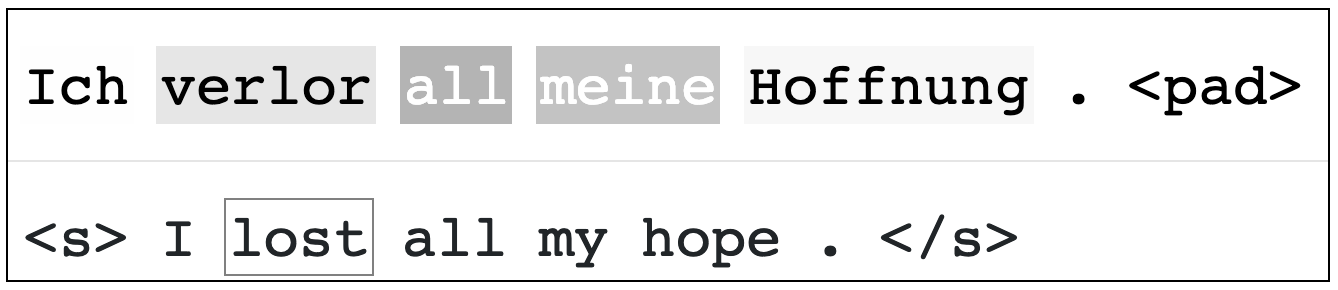
\includegraphics[width=.7\linewidth]{figs/attn1.png}
	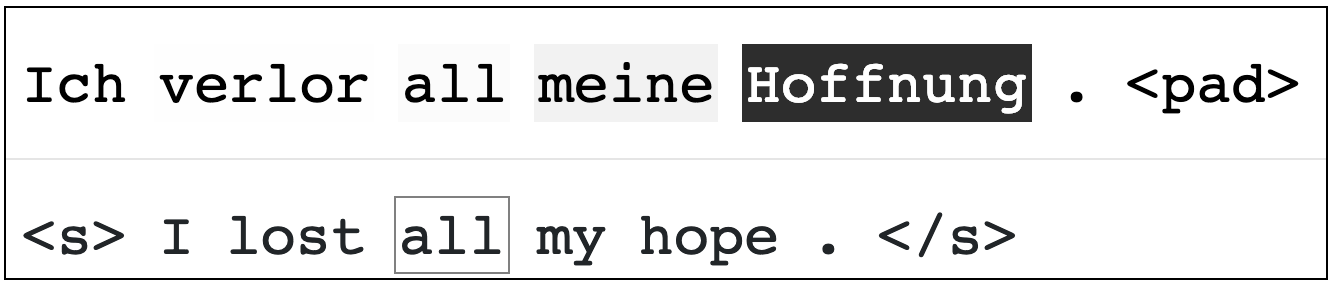
\includegraphics[width=.7\linewidth]{figs/attn2.png}
	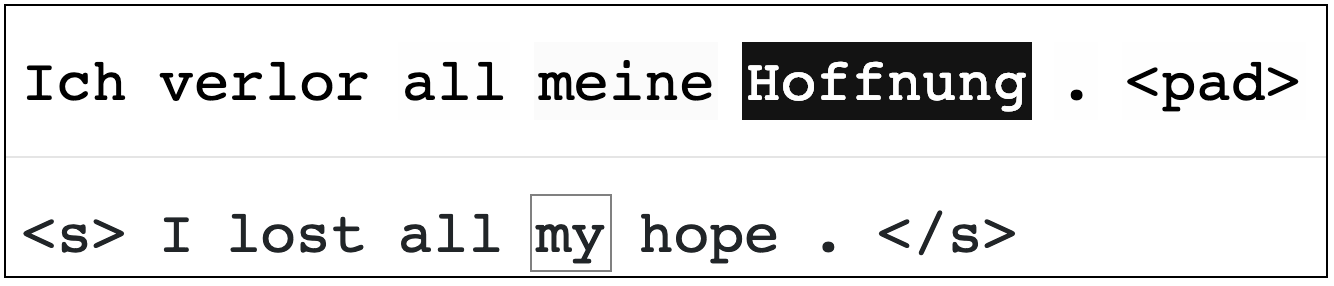
\includegraphics[width=.7\linewidth]{figs/attn3.png}
	\caption{Darker background words signify more attention being placed on that word at each point in the translation process.}
	\label{fig:word_weights}
\end{figure}

\begin{figure}
	\centering
	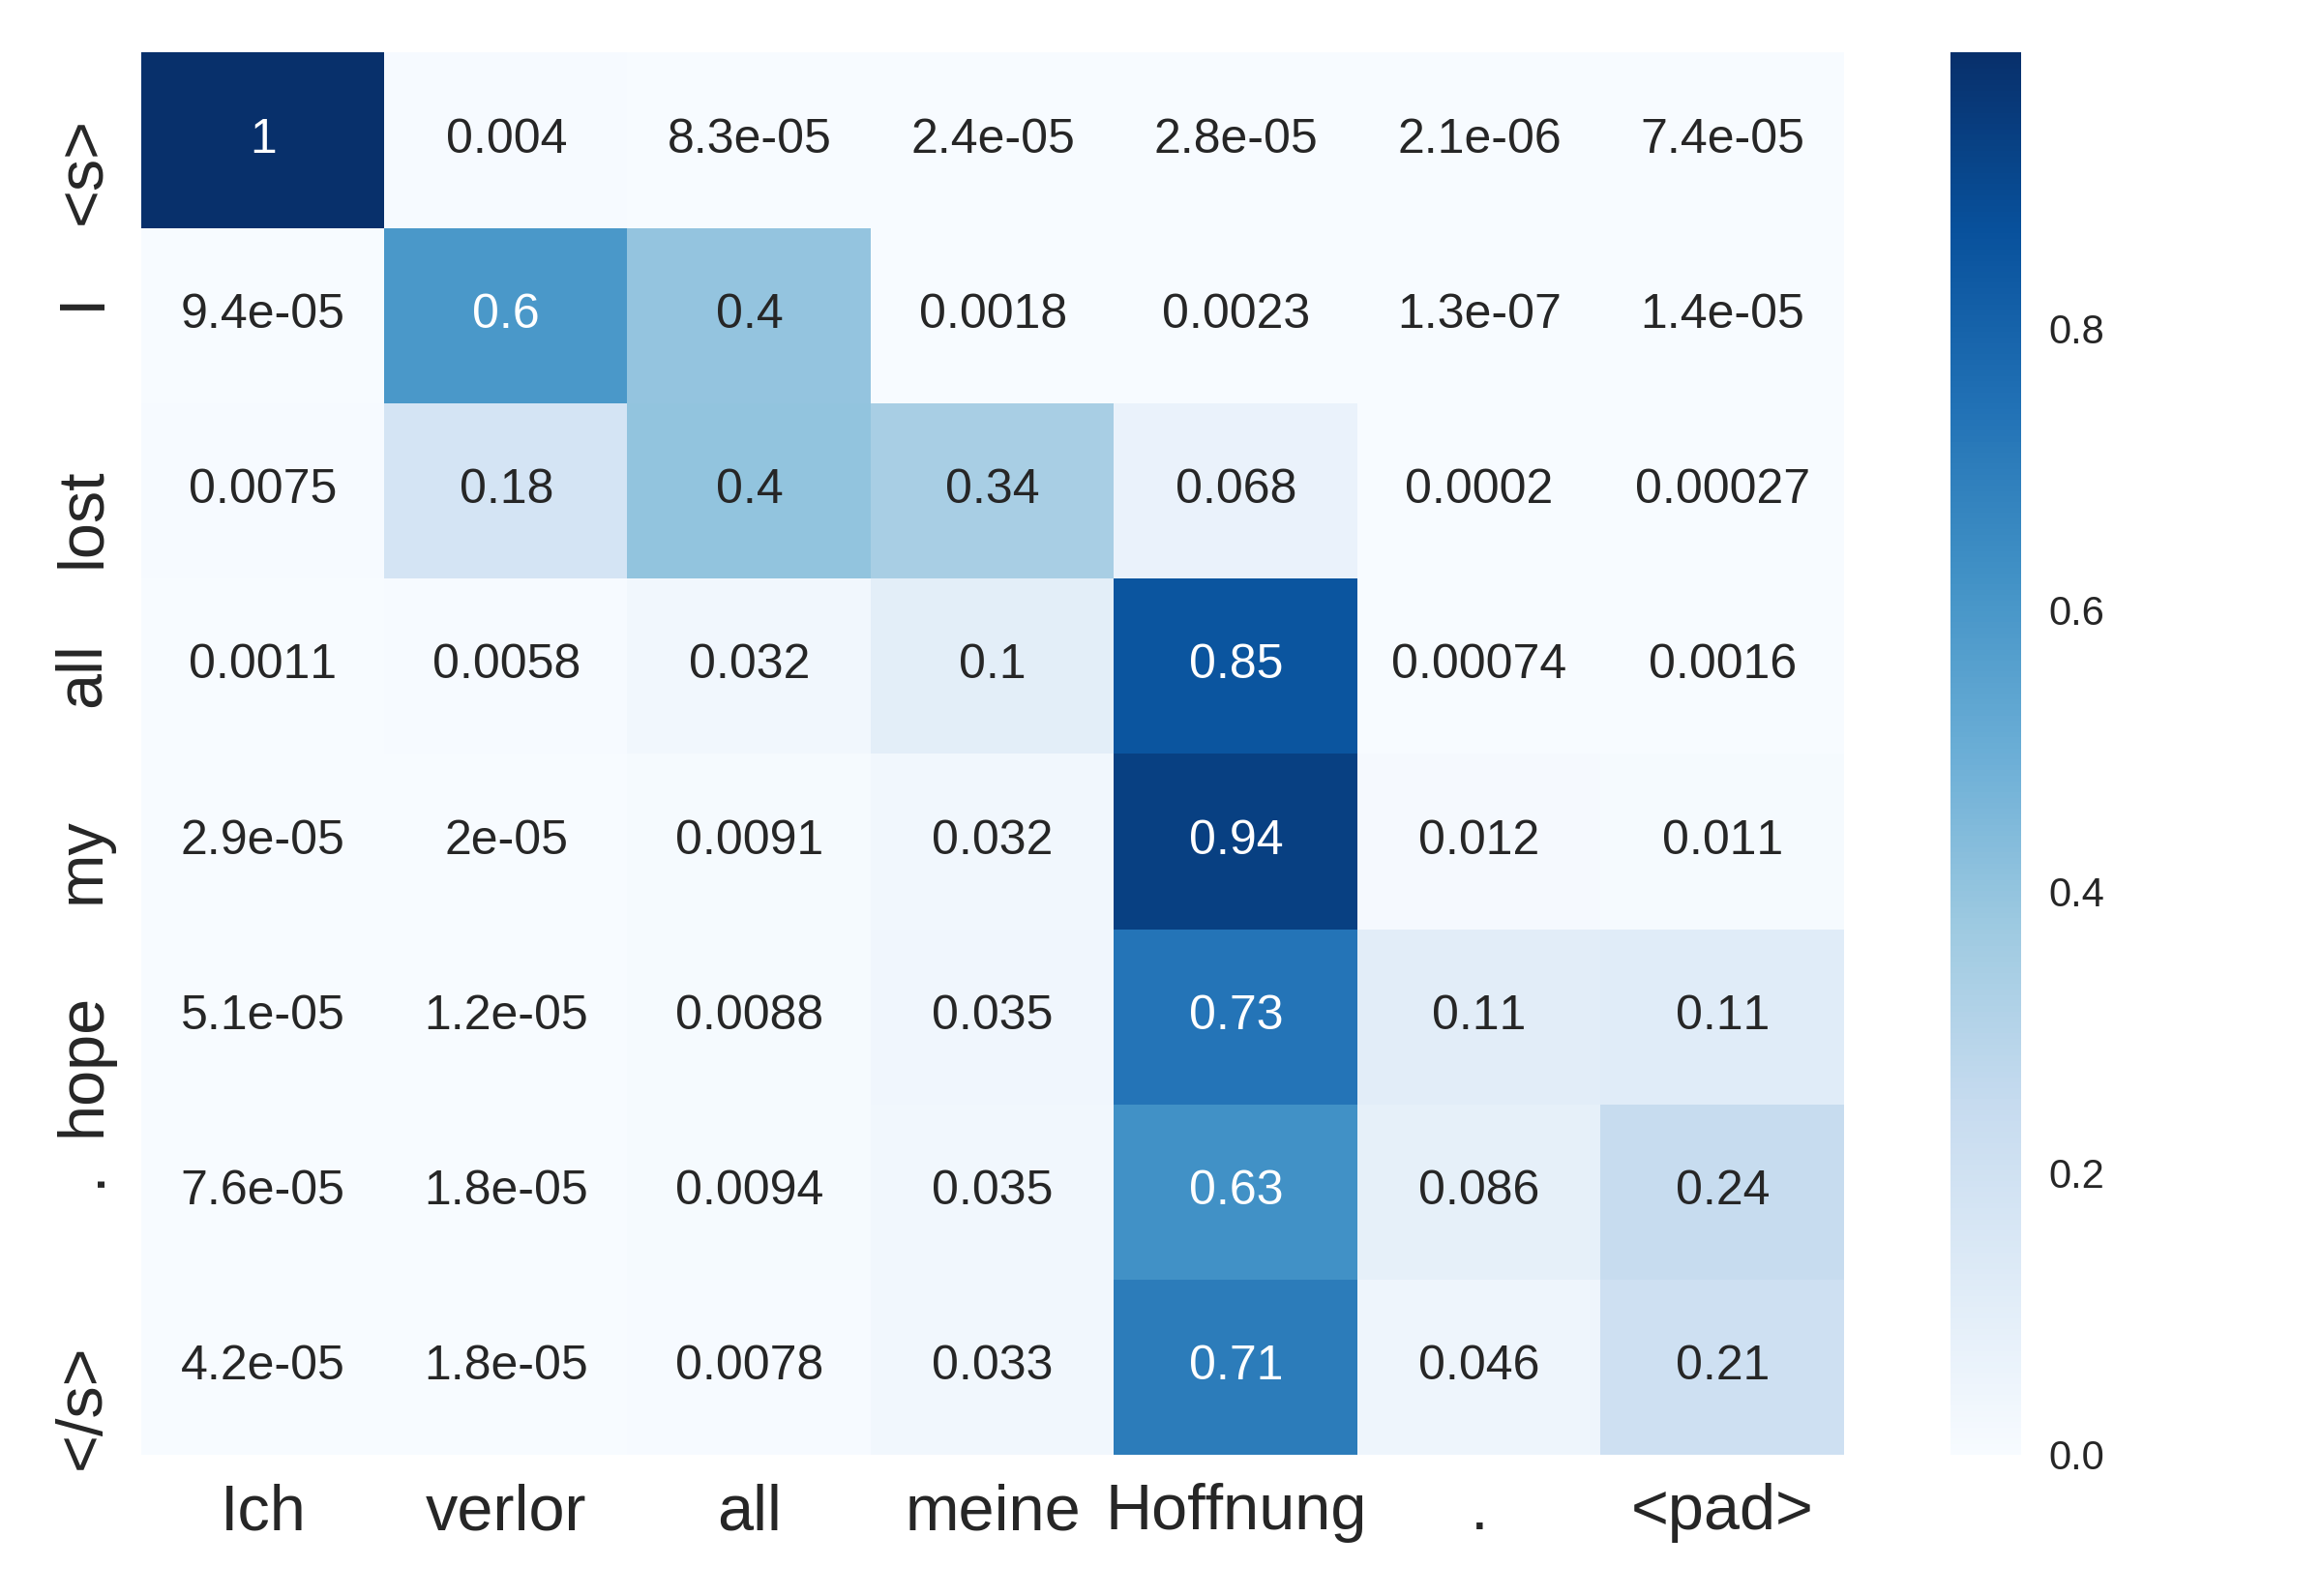
\includegraphics[width=.8\linewidth]{figs/attn_mat.png}
	\caption{Attention matrix weights}
	\label{fig:mat_weights}
\end{figure}

\begin{landscape}
\begin{table}[tb]
    
    \centering
\begin{tabular}{ll}
\toprule
model name                   &specifications\\
\midrule
\texttt{Seq2Seq} & 100 embedding, 100 hidden, no dropout\\
\texttt{Seq2SeqAttn} & Bi-directional LSTM, 100 embedding, 100 hidden, no dropout\\
\bottomrule
\end{tabular}
    \caption{Both models used only one layer in the decoder and trained with Adam and learning rate $10^{-3}$ over 10 epochs. For \texttt{Seq2Seq}, decrease in validation loss flattened at epoch 8. For \texttt{Seq2SeqAttn}, training stopped at epoch 7 after loss starting going up.}
    \label{tab:spec}
\end{table}
\begin{table}[h]
\centering
\begin{tabular}{lrrr}
\toprule
{}                                     & Loss  & Perplexity & BLEU \\
model name                             &       &        & \\
\midrule
\texttt{Seq2Seq}                      & 3.23 & 25.36  & 6.32 \\
\texttt{Seq2SeqAttn}                      & 2.71 & 15.05  & 17.77 \\
\bottomrule
\end{tabular}
\caption{Performance metrics for different models}
\label{table:performance}
\end{table}
\end{landscape}

\bibliographystyle{apalike}
\bibliography{writeup}

\appendix
\section{Model implementation}
\lstinputlisting[caption=Sequence-to-Sequence]{models/seq2seq.py}
\lstinputlisting[caption=LSTM encoder]{models/lstm_encoder.py}
\lstinputlisting[caption=LSTM decoder]{models/lstm_decoder.py}
\lstinputlisting[caption=Attention]{models/attention.py}
\lstinputlisting[caption=Beam search]{models/beam.py}

\end{document}
